\newpage 
\chapter{ آنتن های مایکرواستریپ}
\label{ch:1}

\section{مقدمه}
آنتن‌های مایکرواستریپ به دلیل برخورداری از مزایای متعددی همچون عملکرد مناسب، وزن سبک، قابلیت نصب آسان و هزینه تولید پایین، جایگاه ویژه‌ای در صنایع پیشرفته از جمله هوافضا، ماهواره‌ها و سیستم‌های ارتباطی پیدا کرده‌اند. ساختار چاپی این آنتن‌ها امکان یکپارچه‌سازی آسان با مدارات مایکروویو را فراهم می‌کند. پارامترهای اساسی عملکردی این آنتن‌ها از جمله فرکانس تشدید، الگوی تابشی و امپدانس ورودی عمدتاً توسط ابعاد هندسی پچ، ویژگی‌های زیرلایه و روش تغذیه تعیین می‌شوند. این فصل به ارائه مبانی تئوری، بررسی ویژگی‌ها، مزایا و محدودیت‌های این آنتن‌ها و همچنین تحلیل روش‌های مختلف تغذیه می‌پردازد.
\section{ویژگی های آنتن مایکرواستریپ}


در آنتن‌های مایکرواستریپ، ضخامت پَچ
\LTRfootnote{Patch}
 بسیار نازک است (
$ h \ll \lambda_{0}$
، که 
$ \lambda_{0} $
 طول موج در خلأ است) و ضخامت زیرلایه
\LTRfootnote{Substrate}
  کسری از طول موج است(رابطه 
 \eqref{eq:eq1}
 ). پَچ در بالای لایه زمین قرار گرفته و این دو توسط یک زیرلایه دی‌الکتریک از هم جدا شده‌اند. 
\begin{align}
	\label{eq:eq1}
	0.003\lambda_{0} < h < 0.05\lambda_{0}
\end{align}

در پَچ مستطیلی، اندازه ضلع
\lr{($L$)}
  در محدوده
$ \lambda_{2}/2 < L < \lambda_{2}/3$
    قرار دارد (که
$ \lambda_{2} $
      طول موج در محیط دی‌الکتریک است). ثابت دی‌الکتریک زیرلایه معمولاً در محدوده
$ 2 < \epsilon_r < 12$
        انتخاب میشود. 

پارامترهای زیرلایه تأثیر مستقیمی بر عملکرد آنتن دارند: زیرلایه‌های
\textbf{
 ضخیم‌تر با ثابت دی‌الکتریک پایین‌تر
}
  منجر به
\textbf{
کارایی بالاتر
} 
و
\textbf{
پهنای باند گسترده‌تر
}
میشوند، در حالی که زیرلایه‌های نازک با ثابت دی‌الکتریک بالا موجب
\textbf{
کاهش پهنای باند
}
می‌گردند.


\begin{figure}
\centering
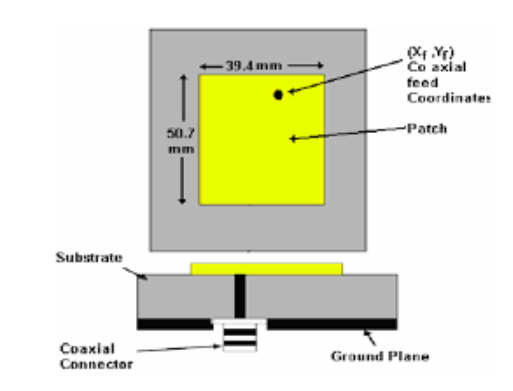
\includegraphics[scale=0.5]{Images/fig1.png}
\caption{پچ مایکرواستریپ با تغذیه ی کواکسیال}
\label{fig1}
\end{figure}
\begin{figure}
	\centering
	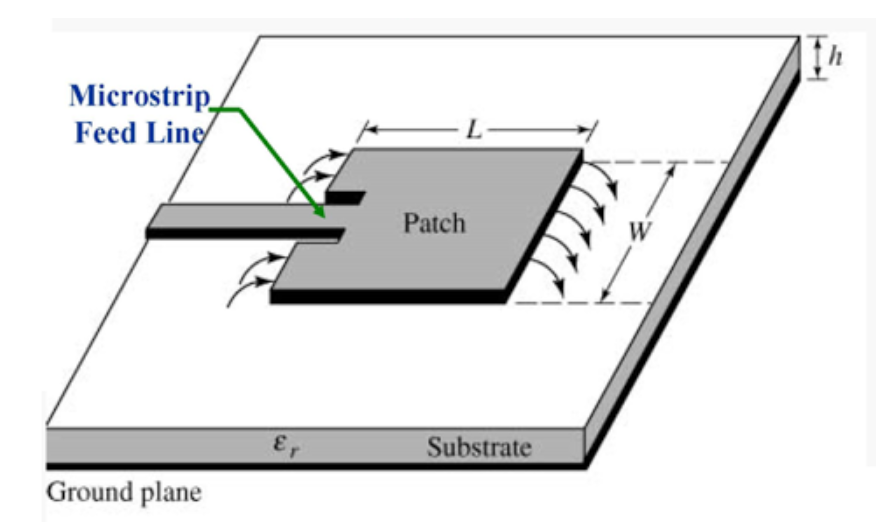
\includegraphics[scale=0.3]{Images/fig2.png}
	\caption{پچ مایکرواستریپ با تغذیه ی خط مایکرواستریپ}
	\label{fig2}
\end{figure}


از میان اشکال مختلف پَچ، انواع مربعی، مستطیلی به دلیل ویژگی‌های تشعشعی مطلوب بیشترین کاربرد را دارند.

\section{معایب آنتن مایکرواستریپ}
بازده پایین، توان پایین، قطبی‌شدگی خالص کم، عملکرد تطبیق ضعیف (فاکتور
$Q$
 بالاتر از ۱۰۰)، تأثیر تغذیه کاذب، و پهنای باند فرکانسی باریک (که در حد یک درصد و در نهایت چند درصد است) را می‌توان از معایب آنتن‌های مایکرواستریپ برشمارد.

البته راهکارهایی مانند افزایش ضخامت زیرلایه، می‌تواند بازده را تا ۹۰ درصد و پهنای باند را تا ۳۵ درصد افزایش دهد. البته با افزایش ضخامت زیرلایه، امواج سطحی
\LTRfootnote{Surface Wave}
 که مطلوب نیستند را نیز باید در نظر گرفت. امواج سطحی به علت تضعیف توان ارسالی مطلوب نیستند. امواج سطحی در زیرلایه انتقال می‌یابند و در ناپیوستگی‌ها و خمیدگی‌ها، مانند نقاط اتصال با صفحه زمین 
\LTRfootnote{Ground Plane}
 ظاهر خواهند شد که مشخصات آنتن (مانند الگوی تشعشع) را تغییر می‌دهد. امواج سطحی وقتی آنتن در یک حفره قرار می‌گیرد قابل صرف‌نظر است.


آنتن مایکرواستریپ خارج از ناحیه عملکرد، اثر الکترومغناطیسی زیادی در فرکانس‌های مشخص خواهد داشت. در سیستم‌های آرایه‌ای حتی در
\lr{VHF}\LTRfootnote{Very High Frequency}
 و
\lr{UHF}\LTRfootnote{Ultra High Frequency}
 بین پهنای باند و نرخ تطبیق، داد و ستد
\LTRfootnote{Trade-off}
  وجود دارد.


\section{انواع تغذیه}
\begin{figure}
	\centering
	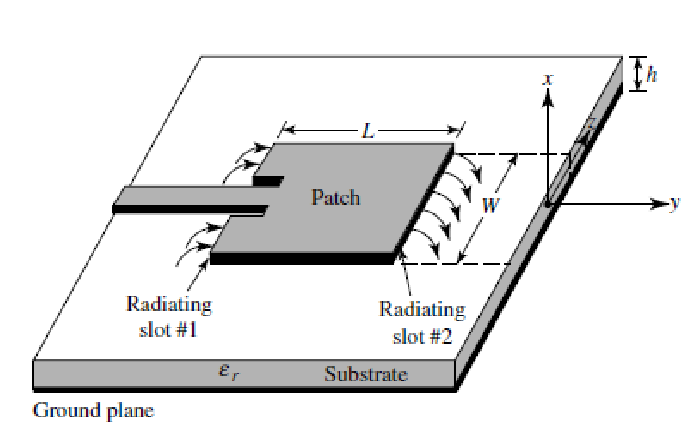
\includegraphics[scale=0.3]{Images/fig3.png}
	\caption{آنتن با تغذیه ی مایکرواستریپ}
	\label{fig3}
\end{figure}
روش‌های متعددی برای تغذیه آنتن‌های مایکرواستریپ وجود دارد که از جمله متداول‌ترین آن‌ها می‌توان به تغذیه توسط خط مایکرواستریپ
\LTRfootnote{Microstrip Line Feed}،
تغذیه کوپلینگ روزنه‌ای
\LTRfootnote{Aperture Coupling}،
 (شکل
\ref{fig4}
)
تغذیه کوپلینگ مجاورتی
\LTRfootnote{Proximity Coupling}
(شکل
\ref{fig5}
)
و تغذیه پروب کواکسیال
\LTRfootnote{Coaxial Probe Feed} 
 (شکل
\ref{fig6}
)
اشاره نمود.  



\subsection{آنتن با تغذیه ی کوپلینگ روزنه ای}
\begin{figure}
	\centering
	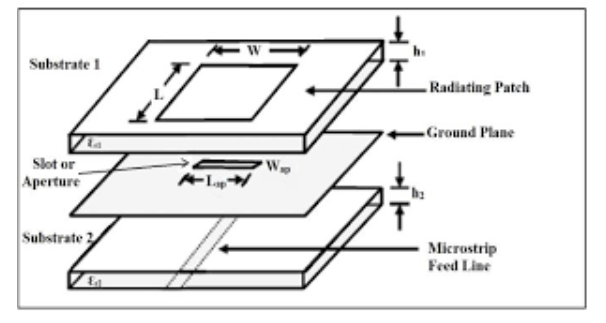
\includegraphics[scale=0.4]{Images/fig4.png}
	\caption{آنتن با تغذیه ی کوپلینگ روزنه ای}
	\label{fig4}
\end{figure}

\subsection{آنتن با تغذیه ی کوپلینگ مجاورتی}
\begin{figure}
	\centering
	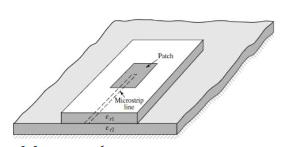
\includegraphics[scale=0.7]{Images/fig5.png}
	\caption{آنتن با تغذیه ی کوپلینگ مجاورتی}
	\label{fig5}
\end{figure}

\subsection{آنتن با تغذیه ی کواکسیال}
در تغذیه آنتن‌های مایکرواستریپ از طریق کابل کواکسیال، هادی مرکزی کابل به پچ و شیلد خارجی کابل به صفحه زمین متصل می‌شود. این روش تغذیه به دلیل سادگی ساخت و امکان تطبیق آسان امپدانس، به طور گسترده‌ای مورد استفاده قرار می‌گیرد. با این حال، این نوع اتصال دارای پهنای باند محدود است و مدل‌سازی دقیق آن در شبیه‌سازی‌ها دشوار می‌باشد.(شکل
\ref{fig6})
\begin{figure}
	\centering
	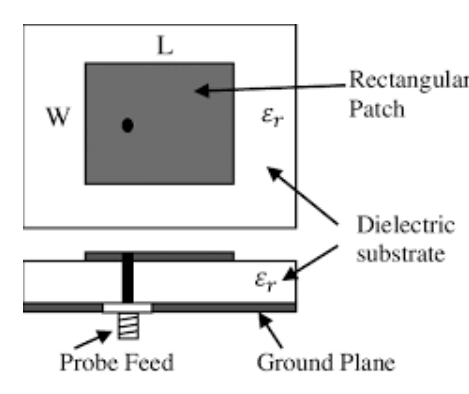
\includegraphics[scale=0.3]{Images/fig6.png}
	\caption{آنتن با تغذیه ی کواکسیال}
	\label{fig6}
\end{figure}


\subsection{آنتن با پچ مستطیلی}
آنتن‌های با پچ مستطیلی به دلیل طراحی ساده، اندازه فشرده و عملکرد پایدار، به‌طور گسترده در سیستم‌های مخابراتی، ماهواره‌ای و راداری مورد استفاده قرار می‌گیرند. در این پژوهش، از روش تغذیه کواکسیال بهره گرفته شده است که در آن هادی مرکزی کابل مستقیماً به پچ و شیلد خارجی به صفحه زمین متصل می‌شود. این روش به دلیل سادگی ساخت، اتلاف پایین و قابلیت تطبیق امپدانس کارآمد، انتخاب شده است؛ هرچند که دارای محدودیت ذاتی در پهنای باند است.(شکل 
\ref{fig7})
\begin{figure}
	\centering
	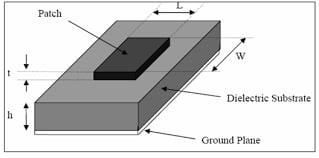
\includegraphics[scale=0.9]{Images/fig7.jpg}
	\caption{آنتن با پچ مستطیلی}
	\label{fig7}
\end{figure}

در این پروژه، از روش تغذیه پروب کواکسیال استفاده شده است که دلیل انتخاب آن، سادگی ساخت، اتلاف کم و قابلیت اطمینان بالا در کاربردهای عملی است. در ادامه، به بررسی دقیق‌تر اصول کاری و ملاحظات طراحی این روش پرداخته خواهد شد.


\section{اثر لبه}

به دلیل محدودیت ابعاد پچ در راستای طول و عرض، میدان‌های الکترومغناطیسی از لبه‌های پچ به بیرون انتشار می‌یابند که این پدیده تحت عنوان اثر لبه‌ای
\LTRfootnote{Fringing Effect}
شناخته می‌شود
\cite{chahar}.
همانطور که در شکل 
\ref{fig8}
نشان داده شده است
\cite{do}،
این اثر منجر به گسترش میدان‌ها در خارج از مرزهای فیزیکی پچ می‌گردد.

\begin{figure}
	\centering
	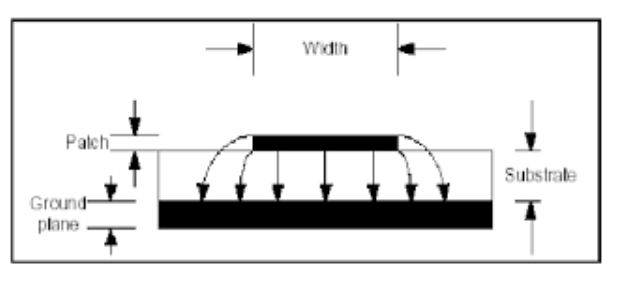
\includegraphics[scale=0.3]{Images/fig8.png}
	\caption{اثر لبه در پچ مایکرواستریپ}
	\label{fig8}
\end{figure}

میزان تراوش میدان از لبه‌ها تابعی از ابعاد هندسی پچ (طول
$L$
 و عرض
$W$)
 و همچنین ویژگی‌های زیرلایه از جمله ارتفاع (
$h$)
 و ثابت دی‌الکتریک (
 $\varepsilon_r$)
 است. برای صفحه اصلی
 $E$،
  این اثر به طور خاص به نسبت
$L$
  و
$\varepsilon_r$
 وابسته می‌باشد.


همانطور که در شکل بالا مشاهده می‌شود، بخش عمده‌ای از خطوط میدان در داخل زیرلایه متمرکز شده‌اند، در حالی که بخشی از آن‌ها به محیط اطراف (هوا) نفوذ می‌کنند. در شرایطی که
$ \frac{W}{h} \gg 1$
 باشد، تراکم خطوط میدان عمدتاً درون زیرلایه رخ می‌دهد. اثر لبه‌ای سبب می‌شود که طول الکتریکی پچ بزرگ‌تر از ابعاد فیزیکی آن به نظر رسد. از آنجایی که بخشی از میدان در هوا و بخشی دیگر در زیرلایه انتشار می‌یابد، یک ثابت دی‌الکتریک مؤثر(
$\varepsilon_{e}$)
 تعریف می‌شود تا تأثیر هر دو محیط به صورت همزمان در محاسبات در نظر گرفته شود. این کمیت به صورت تحلیلی و بر اساس پارامترهای ساختاری آنتن محاسبه شده و نقش اساسی در تعیین دقیق فرکانس تشدید و سایر پارامترهای الکتریکی آنتن ایفا می‌کند.


برای تعریف ثابت دی‌الکتریک موثر، فرض می‌کنیم لایه رسانا با ابعاد اصلی خود (مطابق شکل فوق) در میان زیرلایه قرار گرفته است. ثابت دی‌الکتریکی‌ای که در این حالت، همان مشخصه انتشار حالت قبل را از خود نشان دهد را ثابت دی‌الکتریک موثر(
$\varepsilon_{e}$)
می‌نامند.


اگر ثابت دی‌الکتریک زیرلایه(
$\varepsilon_r$)
بسیار بزرگ باشد، ثابت موثر(
$\varepsilon_{e}$)
به ثابت زیرلایه(
$\varepsilon_{r}$)
نزدیک‌تر است. به علاوه، ثابت موثر تابعی از فرکانس نیز می‌باشد. شکل 
\ref{fig9}
 رابطه بین ثابت موثر دی‌الکتریک و فرکانس را برای سه زیرلایه متفاوت نشان می‌دهد.

\begin{figure}
	\centering
	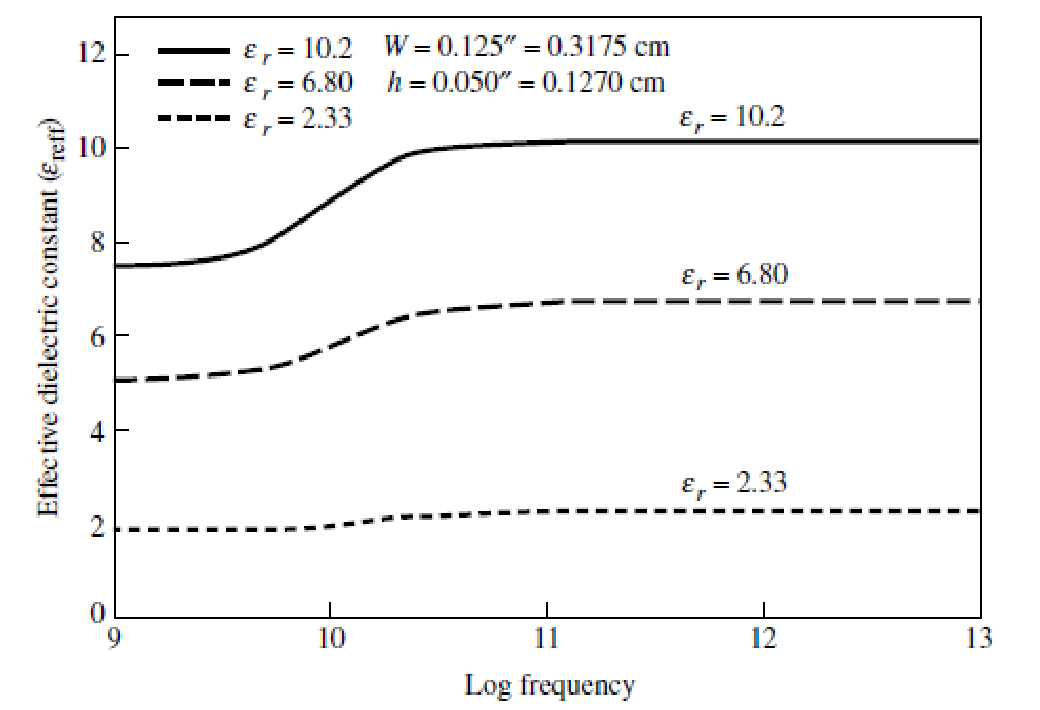
\includegraphics[scale=0.3]{Images/fig9.png}
	\caption{رابطه ی بین ثابت موثر دی الکتریک و فرکانس}
	\label{fig9}
\end{figure}

ثابت موثر دی الکتریک از معادلات 
\ref{eq:eq2}
و
\ref{eq:eq3}
بدست می آید:

\begin{align}
 	\label{eq:eq2}
    \frac{W}{H} < 1	\qquad  \varepsilon_e = \frac{\varepsilon_r+1}{2} + \frac{\varepsilon_r-1}{2} \left[ \left(1+12\frac{H}{W}\right)^{-1/2} + 0.04 \left(1-\frac{W}{H}\right)^2 \right]
\end{align}


\begin{align}
	\label{eq:eq3}
    \frac{W}{H} \geq 1 \qquad \varepsilon_e = \frac{\varepsilon_r+1}{2} + \frac{\varepsilon_r-1}{2} \left(1+12\frac{H}{W}\right)^{-1/2} 
\end{align}


\section{طول موثر، فرکانس تشدید و پهنای باند موثر}
به دلیل اثر حاشیه‌ای
\LTRfootnote{Fringing Effect}،
 طول الکتریکی پَچ به اندازه
$ \delta L$
 افزایش می‌یابد. این افزایش تابعی از ثابت دی‌الکتریک مؤثر(
 $\varepsilon_{e}$)
 و نسبت عرض به ارتفاع
 $W/h$
  زیرلایه است که از رابطه تجربی 
\eqref{eq:eq4}
   محاسبه می‌شود.
\begin{align}
	\label{eq:eq4}
	\frac{\Delta L}{h} = 0.412 \frac{(\varepsilon_{e}+0.3)\left(\frac{W}{h}+0.264\right)}{(\varepsilon_{e}-0.258)\left(\frac{W}{h}+0.8\right)}
\end{align}


\begin{figure}
	\centering
	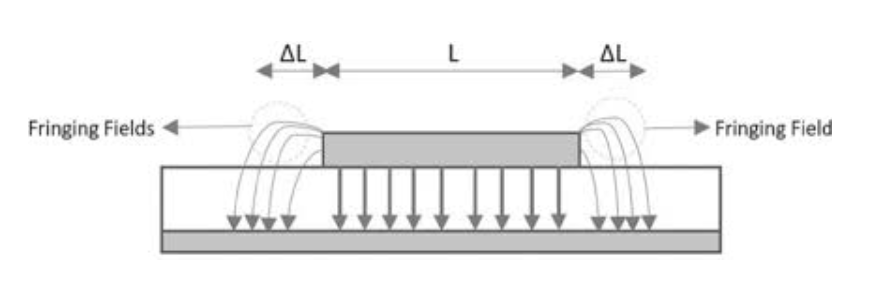
\includegraphics[scale=0.3]{Images/fig10.png}
	\caption{رابطه ی بین ثابت موثر دی الکتریک و فرکانس}
	\label{fig10}
\end{figure}

\begin{figure}
	\centering
	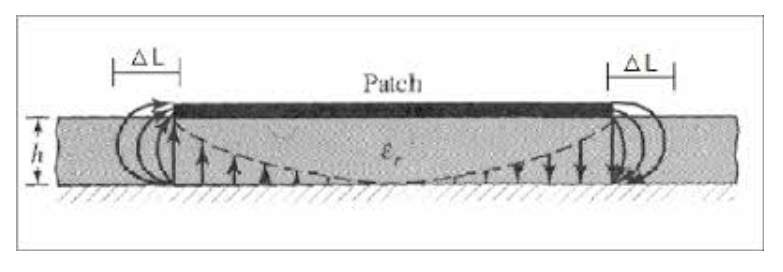
\includegraphics[scale=0.3]{Images/fig11.png}
	\caption{طول های فیزیکی و موثر پچ مایکرواستریپ مستطیلی}
	\label{fig11}
\end{figure}

با در نظر گیری این اثر، طول مؤثر پَچ(
$L_{e}$)
برای محاسبه فرکانس تشدید به صورت 
\eqref{eq:eq5}
 تعریف می‌شود.که در آن 
 $L$
  طول فیزیکی پَچ است.
\begin{align}
	\label{eq:eq5}
	L_{e} = L + 2\delta L
\end{align}

برای مد غالب
$TM_{010}$
فرکانس تشدید به صورت 
\eqref{eq:eq6}
است.
\begin{align}
	\label{eq:eq6}
	(f_r)_{010} = \frac{1}{2L\sqrt{\varepsilon_r}\sqrt{\mu_0\varepsilon_0}} = \frac{v_0}{2L\sqrt{\varepsilon_r}}
\end{align}
$v_0$
سرعت نور در فضای آزاد است.

با در نظرگیری اثر حاشیه‌ای، محاسبه فرکانس تشدید نیازمند اصلاح طول پچ و استفاده از ثابت دی‌الکتریک مؤثر است. فرکانس تشدید برای حالت پایه
$TM_{10}$
 به صورت
\eqref{eq:eq7}
  محاسبه می‌شود.
\begin{align}
	\label{eq:eq7}
	(f_r)_{010} = \frac{1}{2L_{e}\sqrt{\varepsilon_{e}}\sqrt{\mu_0\varepsilon_0}} = \frac{c}{2(L+2\Delta L)\sqrt{\varepsilon_{e}}}
\end{align}

ضریب تراوش
$q$
 به عنوان نسبت فرکانس تشدید واقعی به فرکانس تشدید بدون در نظرگیری اثر حاشیه‌ای به صورت
\eqref{eq:eq8}
  تعریف می‌شود.
\begin{align}
	\label{eq:eq7}
	q = \frac{(f_r)_{\text{actual}}}{(f_r)_{\text{without fringing}}}
\end{align}

با افزایش ارتفاع زیرلایه (
$h$)،
 اثر حاشیه‌ای تشدید شده و موجب افزایش
 $\Delta L$
  و در نتیجه کاهش فرکانس تشدید می‌گردد. این پدیده به‌طور مستقیم بر عملکرد آنتن تأثیر گذاشته و طراحی را به سمت استفاده از مدل‌های دقیق‌تر برای پیش‌بینی رفتار آنتن سوق می‌دهد.











